\documentclass[11pt]{beamer}
\usetheme{JuanLesPins}
\usepackage[utf8]{inputenc}
\usepackage[english]{babel}
\usepackage{amsmath}
\usepackage{amsfonts}
\usepackage{amssymb}
\usepackage{graphicx}
\usepackage{booktabs}
\author{François GUY, Camila Celeste RIBA PEREYRA}
\title{A new introduction to Beamer with \LaTeX}
%\setbeamercovered{transparent} 
%\setbeamertemplate{navigation symbols}{} 
\logo{}
\institute{Université Savoie Mont Blanc, IS-Terre / IREGE} 
\date{\today}
\subject{\LaTeX formation} 
\begin{document}


\section{Introduction}
\begin{frame}[plain]
	\titlepage
\end{frame}

\begin{frame}
\tableofcontents
\end{frame}




\section{Basic facts about ducks}
\subsection{What you need to know immediately}
\begin{frame}{What you need to know immediately 1/2}
	\begin{center}
		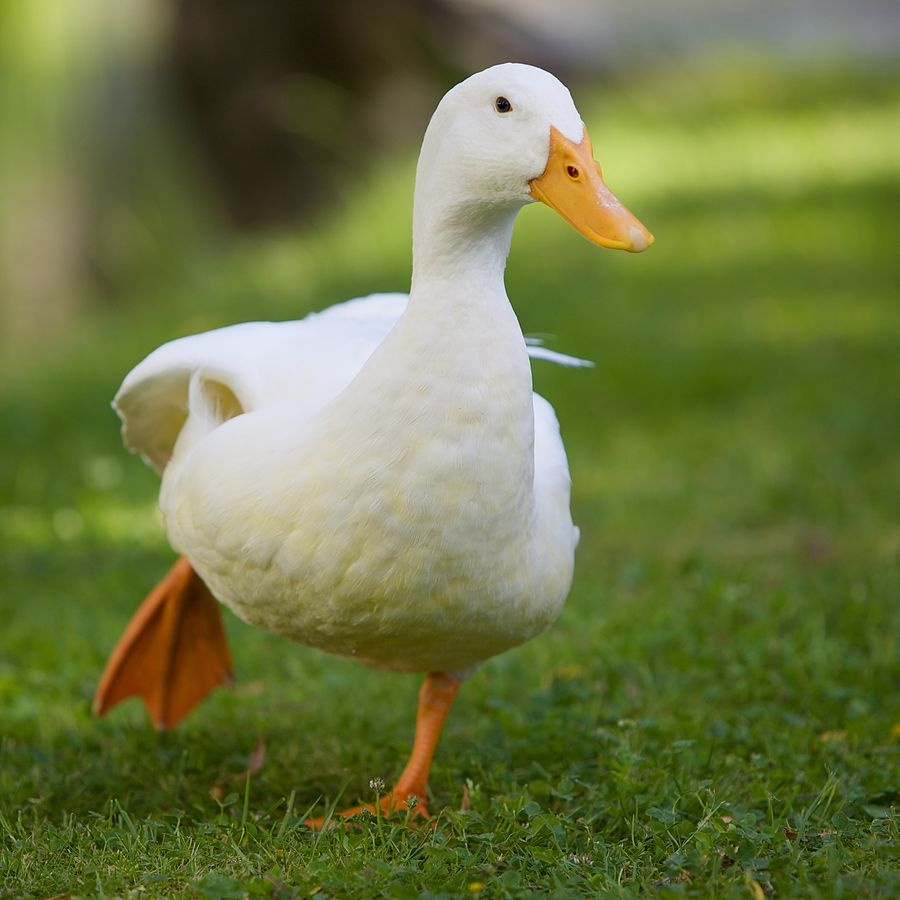
\includegraphics[width = .4\textwidth]{runningduck.jpg}
	\end{center}
	\begin{block} {Useful informations for your everyday life}
		\begin{itemize}
			\pause
			\item Ducks are famous for their hunting skills. They can run up to a speed of 12 feet / second \cite{stewart1958locomotion}
			\pause
			\item They are also famous for their cuteness
		\end{itemize}
	\end{block}
\end{frame}

\begin{frame}{What you need to know immediately 2/2}
	\begin{center}
		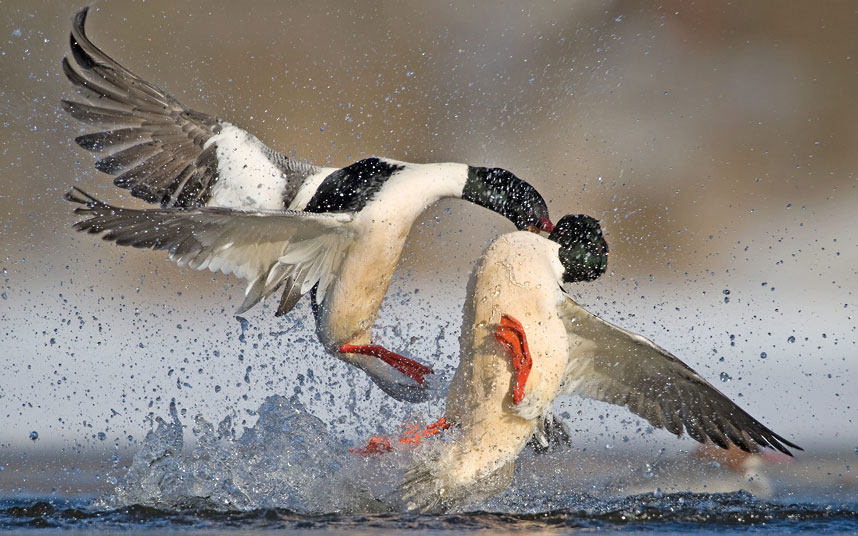
\includegraphics[width = .5\textwidth]{duckfight.jpg}
	\end{center}
	\begin{alertblock} {An alert block}
		\begin{itemize}
			\item Duck can fight up to one opponent !
			\item They are considered  the main cause of bread disappearance in most public parks of Europe
		\end{itemize}
	\end{alertblock}
\end{frame}

\subsection{What you may want to know at one point in your life 1/2}
\begin{frame}{What you may want to know at one point in your life 1/2}
    \begin{columns}[c] % c = Vertical centering
        \column{.6\textwidth}
        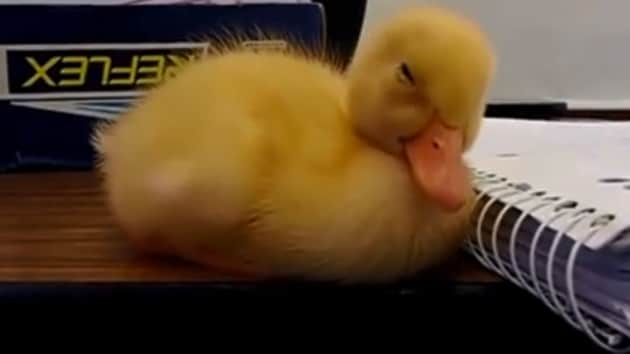
\includegraphics[width = .8\textwidth]{sleepyduck.jpg}
        \column{.4\textwidth}
        \pause
        \begin{block}{Ducklings physical attributes}
            \begin{itemize}
                \item They are even cuter than ducks.
                \item They are even cuter when asleep.
            \end{itemize}
        \end{block}
		\pause
        \begin{block}{Ducklings psychological attributes}
            \begin{itemize}
                \item Sometimes, they bond with a human...
                \item ...Which makes them even more adorable.
            \end{itemize}
        \end{block}
    \end{columns}
\end{frame}




\section{Capybaras}
\begin{frame}{Capybaras fun facts}
	\begin{center}
		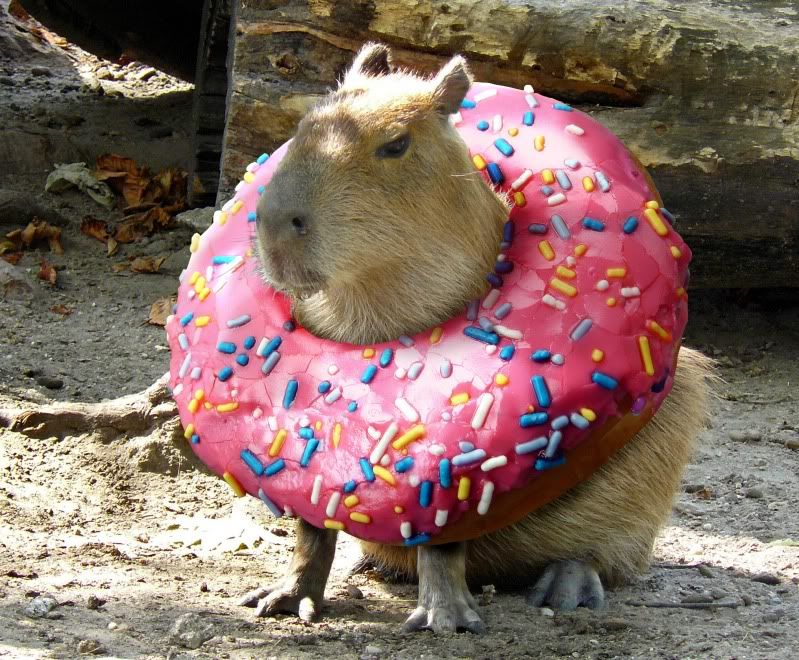
\includegraphics[width = .50\textwidth]{capydonut.jpg}
	\end{center}
	\begin{block} {Did you know?}
		\begin{itemize}
			\item They can run as fast as 35 kph.
			\item Their teeth grow constantly.
		\end{itemize}
	\end{block}
\begin{frame}{What you may want to know at one point in your life 2/2}
\begin{block}{Conclusion of this scientific demonstration}
So yeah, basically, they're just fluffy and cute, but a bit dangerous. What else do you need to know really ?
\end{block}
\end{frame}
\section{Bibliography}

\begin{frame}{Beware with capybaras!}
	\begin{center}
		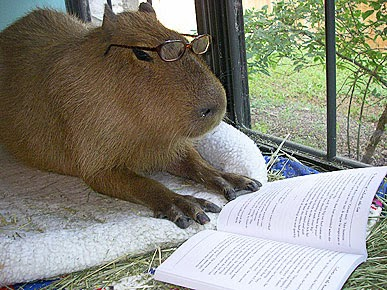
\includegraphics[width = .60\textwidth]{studybara.jpg}
	\end{center}
	\begin{alertblock} {Did you know?}
		\begin{itemize}
			\pause
			\item Capybara eat their own poop, ew!
		\end{itemize}
	\end{alertblock}
\begin{frame}{Bibliography}
\bibliography{bibliography}
\bibliographystyle{apalike}
\end{frame}

\end{document}
